\chapter{Introduction}
\label{introchap}



\section{Background}

Precision landing of spacecraft has 



\section{Motivation}

\section{Literature Review}

COMPARE AND CONTRAST WITH SIMILAR ONLINE MTHODS LIKE LOSSLESS CONVEXIFICAION

COMPARE AND CONTRAST FRAMEWORKW ITH SQP


\section{Research Scope}




In this paper, I present implementations of convex programming algorithms for the powered descent guidance problem. I have implemented the algorithm by Szmuk and Acikmese here \cite{}. I have also used the attitude profiles generated by the algorithm to try a cold gas thruster attitude control system on a cylindrical shaped vehicle mimicking a Vertical-Takeoff-Vertical-Landing (VTVL) rocket.

Having the ability to land near a site of scientific interest, a base, or refueling station is valuable. The convex methods I will present can be used for landing a spacecraft on Mars as well as other planetary bodies like Earth for application in reusable launch vehicles. The ability to soft-land a rocket is fundamentally disruptive to the launch industry and has already had a huge impact in reducing the cost of getting to space. Additionally, similar methods, given navigational upgrades, will be conducive of the development of colonies on other planets. Pin-point landing and divert capability is a necessity in these situations.

Every pinpoint landing problem begins with an entry phase where the vehicle descends through an atmosphere to a point where powered descent must begin. Many Mars entry, descent, and landing schemes enter the atmosphere and slow down via parachute. This parachute is then cut away to allow powered descent. With atmospheric qualities being stochastic, the position in which the descent phase must begin is uncertain. Therefore, we would like to look at algorithms which maximize the divert capability of the craft by minimizing the fuel consumption or final time from initial condition to terminal state. We define powered descent guidance as the generation of a fuel-optimal trajectory that takes the vehicle from some initial state condition to a prescribed final state in a uniform gravitational field with standard vehicle given thrust magnitude and direction constraints.

The convex optimization framework is exploited because it is conducive of real-time on-board implementation and has guaranteed convergence properties with deterministic criteria. The convex programming algorithm to solve powered descent guidance that I will present has non-convex controls constraints and will be posed as a finite-dimensional SOCP problem. SOCPs have low complexity and can be solved in polynomial time \cite{boyd}. Interior-point numerical methods compute optimal solutions with deterministic stopping criteria and are, again conducive to on-board implementation. 


The goal is to be able to generate optimal attitude and translational trajectories. I will use these attitude trajectories later on in a control system implementation.

We shall define the 6DOF minimum final time powered descent problem in the original continuous non-convex dynamic form. The final time of the problem is now an optimization variable. Going forward we will use $t_f$ s the final time of the trajectory, and will refer to this as the time-of-flight.

We shall define our two frames. The $\mathcal{F}_I$ frame defines an inertially fixed Up-East-North reference fram with the origin located at the landing site. The $\mathcal{F}_B$ frame is a body fixed frame follows similarly with the X-axis is aligned vertically with the vehicle, are with the thrust vector at zero gimbal angle. The Y-axis points out of the side of the cylindrical vehicle. The Z-axis completes the right handed triad.














% BELOW THIS LINE ARE TUTORIALS ON THINGS FROM THE TEMPLATE

% \begin{figure}[htbp]
% 	\caption[Cylinder and measurements]{
% 	This diagram of a cylinder and various
% 	measurements and quantities was actually
% 	made using {\bf xfig}, a freeware
% 	drawing program for Unix systems.
% 	Diagrams can be exported directly to PDF
% 	files, the preferred format for
% 	vector graphics.  Vector graphics can
% 	be magnified indefinitely without degradation,
% 	whereas bitmap images (JPG and PNG)
% 	must be pretty high-resolution if you don't
% 	want them looking all pixellated when
% 	magnified.
% 	}
%     \begin{center}
% 	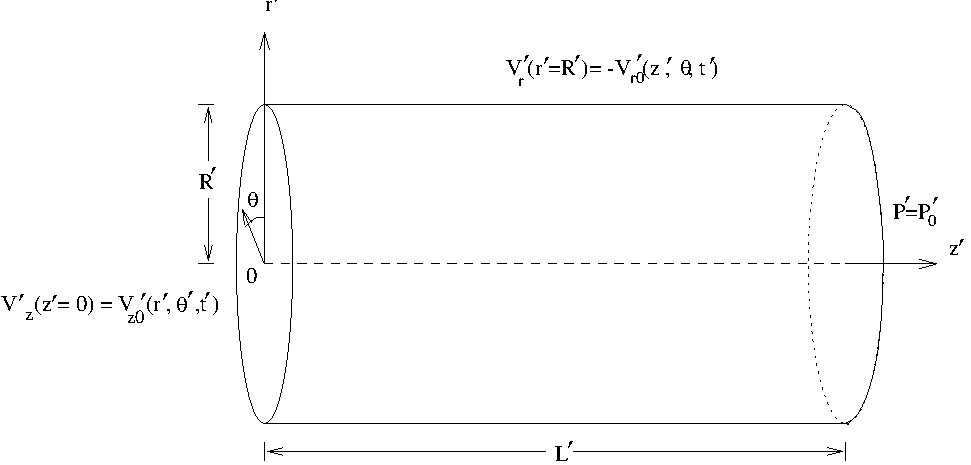
\includegraphics[width=100mm]{figs/cyl.pdf}
%     \end{center}
% \label{xfigDiagram}
% \end{figure}


% \begin{figure}[htbp]
%     \caption[Bitmap images]{
% 	The JPEG bitmap format is great for photos but
% 	crummy for diagrams (including drawings, graphs,
% 	charts) because it can't gracefully handle sharp edges.
% 	Note the same bitmap image below from a PNG file and
% 	from a JPG file; the latter shows characteristic
% 	``ringing'' at sharp edges -- including text!
% 	Seriously, magnify and look closely at the JPG's
% 	awful lines and edges.
% 	Vector-format PDF is the best for diagrams, but
% 	if you must use a bitmap image, let it be PNG.
% 	~ (Left: file {\it drawing.png}.
% 	Right: file {\it drawing.jpg}.)
% 	}
%     \begin{center}
% 	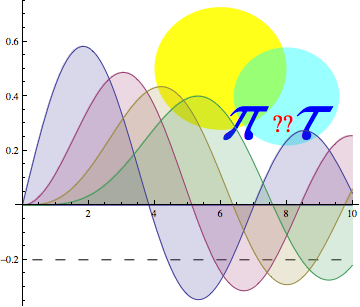
\includegraphics[width=70mm]{figs/drawing.png}
% 	${}^{}$ ~
% 	${}^{}$ ~
% 	${}^{}$
% 	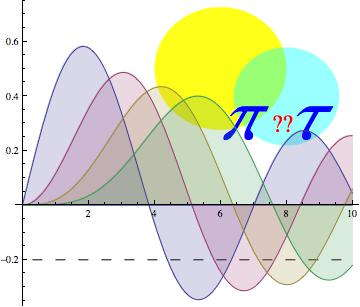
\includegraphics[width=70mm]{figs/drawing.jpg}
%     \end{center}
% \label{bitmapImages}
% \end{figure}



% \section{Lists in {\tt thesis} class}

% In {\tt thesis} class (for Colorado University),
% lists are defined so that nested lists will be
% numbered or marked appropriately.
% First, an itemized (non-enumerated) list
% prefaces each item with a bullet.
% Nested itemized list use asterisks,
% then dashes, then dots.
% These lists are typed between
% the \verb2\begin{itemize}2
% and \verb2\end{itemize}2
% commands.

% \begin{itemize}
%   \item{} This is ``itemized'' item A.
%   \item{} This is ``itemized'' item B.
%   \item{} This is ``itemized'' item C.
%   \begin{itemize}
%     \item{} This is ``itemized'' subitem A.
%     \begin{itemize}
%       \item{} This is ``itemized'' subsubitem A.
%       \begin{itemize}
%         \item{} This is ``itemized'' subsubsubitem A.
%       \end{itemize}
%       \item{} This is ``itemized'' subsubitem B.
%     \end{itemize}
%     \item{} This is ``itemized'' subitem B.
%   \end{itemize}
%   \item{} This is ``itemized'' item D.
% \end{itemize}

% Enumerated lists use the commands
% \verb2\begin{enumerate}2 and
% \verb2\end{enumerate}2,
% and nested enumerations appear like this.

% \begin{enumerate}
%   \item{} This is ``enumerated'' item A.
%   \item{} This is ``enumerated'' item B.
%   \item{} This is ``enumerated'' item C.
%   \begin{enumerate}
%     \item{} This is ``enumerated'' subitem A.
%     \begin{enumerate}
%       \item{} This is ``enumerated'' subsubitem A.
%       \begin{enumerate}
%         \item{} This is ``enumerated'' subsubsubitem A.
%       \end{enumerate}
%       \item{} This is ``enumerated'' subsubitem B.
%     \end{enumerate}
%     \item{} This is ``enumerated'' subitem B.
%   \end{enumerate}
%   \item{} This is ``enumerated'' item D.
% \end{enumerate}


% The work presented
% here\footnote{Footnotes are handled neatly by \LaTeX.}
% is an extension of Lao\cite{lao:thesis}
% and Lao et~al.\cite{lao:paper},
% fictional references that are in the bibliographic
% source file \verb9refs.bib9.

% \begin{table}[htb]
%     \caption[Example of a table with its own footnotes]{
% 	Here is an example of a table with its own footnotes.
% 	Don't use the $\backslash${\tt footnote} macro if you
% 	don't want the footnotes at the bottom of the page.
% 	Also, note that in a thesis the caption goes
% 	\emph{above} a table, unlike figures.
% 	}
%     \begin{center}
%     \begin{tabular}{||l|c|c|c|c||} \hline
% 	& $S$ & $P$ &   $Q^{\ast}$  & $D^{\dagger}$ \\	% footnote symbols!
% 	wave form & (kVA) & (kW) & (kVAr) & (kVAd) \\  \hline \hline
% 	Fig.  \ref{xfigDiagram}a  & 25.48 & 25.00 & -2.82 & 4.03 \\ \hline
% 	Fig.  \ref{xfigDiagram}b  & 25.11 & 18.02 & -9.75 & 14.52 \\ \hline
% 	Table \ref{pdftable}  & 24.98 & 22.26 & 9.19 & 6.64 \\ \hline
% 	Table \ref{powertable}  & 23.48 & 15.00 & 6.59 & 16.82 \\ \hline
% 	Fig.  \ref{pyramid}  & 24.64 & 22.81 & -0.44 & 9.3 \\ \hline
% 	\end{tabular}
%    \\ \rule{0mm}{5mm}
%    ${}^\ast$kVAr means reactive power.		% footnote symbol
% \\ ${}^\dagger$kVAd means distortion power.	% footnote symbol
% \end{center}
% \label{powertable}
% \end{table}


